\chapter{Arhitektura i dizajn sustava}

\subsection{Opis arhitekture}

\textit{Detaljnom razradom cilja projektnog zadatka, u kojem je fokus izrada aplikacije za iznajmljivanje električnih romobila, definirali smo razinu klijenta, razinu web-aplikacije te sloj pristupa podatcima kao osnovne razine naše aplikacije.}

\subsubsection{Razina klijenta}

\textit{Razina klijenta predstavlja korisničko sučelje web-aplikacije koje korisnici vide i s kojim interagiraju. U razvoju projekta korišten je React, odnosno JavaScript knjižica za izradu korisničkog sučelja. Organizirano je u komponente koje predstavljaju određene dijelove korisničkog sučelja. Korišten je virtualni DOM (Document Object Model), kojim se ubrzava proces ažuriranja promjena korisničkog sučelja u svrhu poboljšavanja performansi web-aplikacije. }
\subsubsection{Razina web-aplikacije}

\textit{Sloj web-aplikacije je odgovoran za obradu zahtjeva korisnika, poslovnu logiku i komunikaciju s bazom podataka. U razvoju projekta korišten je okvir za razvoj web aplikacija Spring Boot u programskom jeziku Java. U Spring Bootu, kontroleri su odgovorni za obradu HTTP zahtjeva i usmjeravanje na odgovarajuće servise za obradu zahtjeva. Obradu podataka, validaciju te logiku obavljaju servisi, dok modeli predstavljaju strukturu podataka koja se koristi za komunkaciju s bazom podataka te prenošenje podataka između kontrolera i servisa.}
\subsubsection{Sloj pristupa podatcima}

\textit{Sloj pristupa podacima je odgovoran za komunikaciju s bazom podataka i pristupanje podacima. Građen je od entiteta s vlastitim atributima koji predstavljaju modele podataka koji odgovaraju tablicama u bazi podataka.}

\textit{Sinteza ovih slojeva - korisničkog sučelja na razini Reacta, web-aplikacijskog sloja u Spring Bootu i sloja pristupa podacima u Spring Bootu - stvara temelj za razvoj visoko skalabilnih i funkcionalnih web-aplikacija. Korisnici ostvaruju interakciju s aplikacijom preko intuitivnog React korisničkog sučelja, dok Spring Boot preuzima odgovornost za obradu njihovih zahtjeva i poslovne logike. Istovremeno, sloj pristupa podacima omogućuje efikasnu komunikaciju s bazom podataka, omogućujući pohranu i dohvat podataka s pouzdanošću i učinkovitošću.}

\subsection{MVC arhitektura}
\textit{Model-View-Controller (MVC) je arhitekturni obrazac koji se koristi za organizaciju komponenti u softverskim aplikacijama, posebno u razvoju web-aplikacija. Osnovna svrha MVC-a je odvajanje različitih aspekata aplikacije kako bi se omogućila bolja organizacija, održavanje i skalabilnost. Sastoji se od tri glavne komponente:}
\begin{itemize}
	\item\textit{Model - predstavlja sloj koji je odgovoran za obradu podataka i poslovnu logiku aplikacije te sadrži podatke i pravila za njihovu obradu.}
	\item\textit{View - predstavlja sloj koji se odnosi na korisničko sučelje aplikacije i odgovoran je za prikazivanje podataka korisnicima. Ne obavlja nikakvu poslovnu logiku, samo prikazuje podatke koji mu se dostave iz modela.}
	\item\textit{Kontroler - posrednik između Model i View komponenti. Prima korisničke zahtjeve, obrađuje ih te komunicira s Modelom radi dohvaćanja ili ažuriranja podataka. Također, odlučuje koji View treba biti prikazan korisniku na temelju podataka iz Modela te korisničkih zahtjeva, upravlja tokom aplikacije te sadrži logiku za validaciju, autorizaciju i upravljanje sesijama.}
\end{itemize}

\textit{MVC arhitektura omogućuje precizno razgraničenje odgovornosti unutar aplikacije. Ovo strukturalno odvajanje olakšava razvoj aplikacije, čini ju lakšom za održavanje i omogućava efikasnije testiranje. Svaka od tri glavne komponente - Model, View i Controller - može se ponovno koristiti na različitim dijelovima aplikacije. To potiče efikasnost razvoja jer se već razvijeni dijelovi aplikacije mogu lako iskoristiti u drugim kontekstima. MVC omogućuje skalabilnost aplikacije jer se jasno razdvajaju različiti aspekti. Novi dijelovi funkcionalnosti mogu se dodavati bez narušavanja postojeće arhitekture, što omogućava aplikaciji da raste i prilagodi se promjenama. }


\section{Baza podataka}

\textit{U kontekstu našeg sustava, baza podataka igra ključnu ulogu, pružajući strukturiranu platformu za modeliranje stvarnog svijeta. Temeljni građevni blok ove baze je relacija, odnosno tablica koja je jasno definirana svojim imenom i skupom atributa. Glavna svrha baze podataka je olakšati brzu i jednostavnu pohranu, promjenu te izvlačenje podataka kako bi se omogućila daljnja analiza i obrada. Unutar baze podataka za našu aplikaciju, identificiramo nekoliko ključnih entiteta:
	\begin{itemize}
		\item 	\textit{User}
		\item 	\textit{Preferences}
		\item 	\textit{SocialMedia}
		\item 	\textit{PrivacySettings}
		\item 	\textit{Document}
		\item 	\textit{Scooter}
		\item 	\textit{Listing}
		\item 	\textit{Review}
		\item 	\textit{Transaction}
		\item 	\textit{Invoice}
		\item 	\textit{Notification}
		\item 	\textit{ChatSession}
		\item 	\textit{Message}
		\item 	\textit{ImageChangeRequest}
	\end{itemize}
}

\subsection{User}


\textit{Ovaj entitet sadrzava sve važne informacije o korisniku aplikacije. Sadrži atribute: userId, nickname, firstName, lastName, cardNumber, email, phoneNumber, password, role te status. Ovaj entitet ima One-to-one vezu s entitetom Preferences preko atributa userId, One-to-one vezu s entitetom PrivacySettings preko atributa userId, One-to-one vezu s entitetom SocialMedia preko atributa userId, One-to-many vezu s entitetom Documents preko atributa userId, One-to-many vezu s entitetom Scooters preko atributa userId, One-to-many vezu s entitetom Listings preko atributa renterUsername, One-to-many vezu s entitetom Reviews preko atributa reviewerUsername, One-to-many vezu s entitetom ChatSessions preko atributa user1 ili atributa user2, One-to-many vezu s entitetom Messages preko atributa senderUsername, One-to-many vezu s entitetom ImageChangeRequest preko atributa requesterId te One-to-many vezu s entitetom Notifications preko atributa userId, requestingUser te decisionAdmin.}


\begin{longtblr}[
	label=none,
	entry=none
]{
	width = \textwidth,
	colspec={|X[6,l]|X[6, l]|X[20, l]|},
	rowhead = 1,
} %definicija širine tablice, širine stupaca, poravnanje i broja redaka naslova tablice
	\hline \SetCell[c=3]{c}{\textbf{User}}	 \\ \hline[3pt]
	\SetCell{LightGreen}userId & INT	&  jedinstveni identifikator korisnika	\\ \hline
	nickname	& VARCHAR &  jedinstveni nadimak korisnika  	\\ \hline
	firstName & VARCHAR &  ime korisnika  \\ \hline
	lastName & VARCHAR	& prezime korisnika
	\\ \hline
	cardNumber	& INT &   broj kartice korisnika	\\ \hline
	email	& VARCHAR &    jedinstvena email adresa korisnika	\\ \hline
	phoneNumber	& INT &   jedinstveni kontakt broj korisnika 	\\ \hline
	password	& VARCHAR & zaporka za prijavu korisnika   	\\ \hline
	role	& UserRole &  uloga korisnika ('unregistered', 'registered', 'renter', 'admin') 	\\ \hline
	status	& UserStatus & status korisnika ('pending', 'rejected', 'accepted', 'blocked') 	\\ \hline
\end{longtblr}

\subsection{Preferences}


\textit{Ovaj entitet sadrzava sve važne informacije o preferencama korisnika aplikacije. Sadrži atribute: userId, language i darkMode. Ovaj entitet ima One-to-one vezu s entitetom User preko atributa userId,}


\begin{longtblr}[
	label=none,
	entry=none
]{
	width = \textwidth,
	colspec={|X[6,l]|X[6, l]|X[20, l]|},
	rowhead = 1,
} %definicija širine tablice, širine stupaca, poravnanje i broja redaka naslova tablice
	\hline \SetCell[c=3]{c}{\textbf{Preferences}}	 \\ \hline[3pt]
	\SetCell{LightGreen}userId & INT	&  jedinstveni identifikator korisnika	 	\\ \hline
	language	& UserLanguage & jezik korisnika   	\\ \hline
	darkMode & BOOLEAN &  omogućen dark mode \\ \hline
\end{longtblr}

\subsection{Social Media}


\textit{Ovaj entitet sadrzava sve važne informacije o socijalnim mrežama korisnika aplikacije. Sadrži atribute: userId, instagram, facebook, google i tikTok. Ovaj entitet ima One-to-one vezu s entitetom User preko atributa userId.}


\begin{longtblr}[
	label=none,
	entry=none
]{
	width = \textwidth,
	colspec={|X[6,l]|X[6, l]|X[20, l]|},
	rowhead = 1,
} %definicija širine tablice, širine stupaca, poravnanje i broja redaka naslova tablice
	\hline \SetCell[c=3]{c}{\textbf{Social Media}}	 \\ \hline[3pt]
	\SetCell{LightGreen}userId & INT	&  jedinstveni identifikator korisnika	 	\\ \hline
	instagram	& VARCHAR &   	\\ instagram account korisnika \hline
	facebook & VARCHAR & facebook account korisnika  \\ \hline
	google & VARCHAR	&  google account korisnika		\\ \hline
	tikTok	& VARCHAR &  tikTok account korisnika 	\\ \hline
\end{longtblr}

\subsection{PrivacySettings}


\textit{Ovaj entitet sadrzava sve važne informacije o postavkama privatnosti korisnika aplikacije. Sadrži atribute: userId, isFirstNameVisible, isLastNameVisible, isNicknameVisible i isEmailVisible. Ovaj entitet ima One-to-one vezu s entitetom User preko atributa userId.}


\begin{longtblr}[
	label=none,
	entry=none
]{
	width = \textwidth,
	colspec={|X[6,l]|X[6, l]|X[20, l]|},
	rowhead = 1,
} %definicija širine tablice, širine stupaca, poravnanje i broja redaka naslova tablice
	\hline \SetCell[c=3]{c}{\textbf{Privacy Settings}}	 \\ \hline[3pt]
	\SetCell{LightGreen}userId & INT	&  	 jedinstveni identifikator korisnika	\\ \hline
	isFirstNameVisible	& BOOLEAN &   omogućena vidljivost imena korisnika	\\ \hline
	isLastNameVisible & BOOLEAN &   \\ omogućena vidljivost prezimena korisnika\hline
	isNicknameVisible & BOOLEAN	&  		omogućena vidljivost nadimka korisnika\\ \hline
	isEmailVisible & BOOLEAN	&  		omogućena vidljivost emaila korisnika\\ \hline
\end{longtblr}

\subsection{Document}


\textit{Ovaj entitet sadrzava sve važne informacije o dokumentima korisnika aplikacije. Sadrži atribute: userId, documentType, url i status. Ovaj entitet ima One-to-one vezu s entitetom User preko atributa userId.}


\begin{longtblr}[
	label=none,
	entry=none
]{
	width = \textwidth,
	colspec={|X[6,l]|X[6, l]|X[20, l]|},
	rowhead = 1,
} %definicija širine tablice, širine stupaca, poravnanje i broja redaka naslova tablice
	\hline \SetCell[c=3]{c}{\textbf{Document}}	 \\ \hline[3pt]
	\SetCell{LightGreen}userId & INT	&  jedinstveni identifikator korisnika	 	\\ \hline
	documentType	& DocumentType &  tip dokumenta ('criminalRecord', 'identification')	\\ \hline
	url & VARCHAR &  url dokumenta \\ \hline
	status & DocumentStatus	& status dokumenta ('pending', 'approved', 'rejected') 		\\ \hline
\end{longtblr}

\subsection{Scooter}


\textit{Ovaj entitet sadrzava sve važne informacije o pojedinom romobilu. Sadrži atribute:scooterId, manufacturer, model, batteryCapacity, maxSpeed, imageUrl, maxRange, yearOfManufacture, additionalInformation, userId i availability. Ovaj entitet ima One-to-one vezu s entitetom User preko atributa userId te One-to-many vezu s entitetom Listings preko atributa scooterId.}


\begin{longtblr}[
	label=none,
	entry=none
]{
	width = \textwidth,
	colspec={|X[6,l]|X[6, l]|X[20, l]|},
	rowhead = 1,
} %definicija širine tablice, širine stupaca, poravnanje i broja redaka naslova tablice
	\hline \SetCell[c=3]{c}{\textbf{Scooter}}	 \\ \hline[3pt]
	\SetCell{LightGreen}scooterId & INT	&  	jedinstveni identifikator romobila 	\\ \hline
	manufacturer	& VARCHAR & proizvođač romobila  	\\ \hline
	model & VARCHAR &  model romobila \\ \hline
	batteryCapacity & INT	& kapacitet baterije 		\\ \hline
	maxSpeed 	& INT &   maksimalna brzina	\\ \hline
	imageUrl	& TEXT &  url slike 	\\ \hline
	maxRange	& FLOAT & maksimalni domet  	\\ \hline
	yearOfManufacture	& INT &   	godina proizvodnje\\ \hline
	additionalInformation	& TEXT &  dodatne informacije 	\\ \hline
	userId	& INT & jedinstveni identifikator korisnika  	\\ \hline
	\SetCell{LightBlue}availability	& BOOLEAN &  dostupnost 	\\ \hline
\end{longtblr}

\subsection{Listing}


\textit{Ovaj entitet sadrzava sve važne informacije o pojedinom oglasu. Sadrži atribute:listingId, currentAddress, returnAddress, returnByTime, pricePerKilometer, penaltyFee, scooterId, listingTime, notes i status. Ovaj entitet ima One-to-one vezu s entitetom Scooter preko atributa scooterId, One-to-many vezu s entitetom Reviews preko atributa transactionId te One-to-many vezu s entitetom Transactions preko atributa listingId.}


\begin{longtblr}[
	label=none,
	entry=none
]{
	width = \textwidth,
	colspec={|X[6,l]|X[6, l]|X[20, l]|},
	rowhead = 1,
} %definicija širine tablice, širine stupaca, poravnanje i broja redaka naslova tablice
	\hline \SetCell[c=3]{c}{\textbf{Listing}}	 \\ \hline[3pt]
	\SetCell{LightGreen}listingId & INT	&  jedinstveni identifikator oglasa	 	\\ \hline
	currentAddress	& VARCHAR & trenutna adresa  	\\ \hline
	returnAddress & VARCHAR	& adresa povratka 		\\ \hline
	returnByTime 	& TIMESTAMP & vrijeme vraćanja   	\\ \hline
	pricePerKilometer	& FLOAT &   cijena po kilometru	\\ \hline
	penaltyFee	& FLOAT &   	kaznena naknada\\ \hline
	\SetCell{LightBlue}scooterId	& INT &  jedinstveni identifikator romobila 	\\ \hline
	listingTime	& TIMESTAMP &   	vrijeme objave oglasa\\ \hline
	notes	& TEXT &  bilješke 	\\ \hline
	status	& ListingStatus &   	status oglasa ('active', 'finished', 'cancelled')\\ \hline
\end{longtblr}

\subsection{Review}


\textit{Ovaj entitet sadrzava sve važne informacije o pojedinom osvrtu. Sadrži atribute: transactionId, reviewerUsername, renterUsername, stars, comment te reviewTime. Ovaj entitet ima Many-to-one vezu s entitetom User preko atributa reviewerUsername, Many-to-one vezu s entitetom User preko atributa renterUsername te One-to-one vezu s entitetom Transaction preko atributa transactionId.}


\begin{longtblr}[
	label=none,
	entry=none
]{
	width = \textwidth,
	colspec={|X[6,l]|X[6, l]|X[20, l]|},
	rowhead = 1,
} %definicija širine tablice, širine stupaca, poravnanje i broja redaka naslova tablice
	\hline \SetCell[c=3]{c}{\textbf{Review}}	 \\ \hline[3pt]
	\SetCell{LightGreen}transactionId & INT	&  jedinstveni identifikator transakcije	 	\\ \hline
	\SetCell{LightBlue}reviewerUsername	& VARCHAR &  korisničko ime recenzenta 	\\ \hline
	\SetCell{LightBlue}renterUsername & VARCHAR &  korisničko ime iznajmljivača \\ \hline
	stars & INT	&  	broj zvjezdica/ocjena	\\ \hline
	comment	& TEXT &  komentar 	\\ \hline
	reviewTime	& TIMESTAMP &   vrijeme osvrta	\\ \hline
\end{longtblr}

\subsection{Transaction}


\textit{Ovaj entitet sadrzava sve važne informacije o pojedinoj transakciji. Sadrži atribute: transactionId, kilometersTraveled, totalPrice, listingId, paymentTime te previousTransactionStatus. Ovaj entitet ima One-to-one vezu s entitetom Listing preko atributa listingId te One-to-one vezu s entitetom Invoice preko atributa transactionId.}


\begin{longtblr}[
	label=none,
	entry=none
]{
	width = \textwidth,
	colspec={|X[6,l]|X[6, l]|X[20, l]|},
	rowhead = 1,
} %definicija širine tablice, širine stupaca, poravnanje i broja redaka naslova tablice
	\hline \SetCell[c=3]{c}{\textbf{Transaction}}	 \\ \hline[3pt]
	\SetCell{LightGreen}transactionId & INT	&  jedinstveni identifikator transakcije	 	\\ \hline
	kilometersTraveled	& FLOAT &   broj prijeđenih kilometara	\\ \hline
	totalPrice	& FLOAT &   ukupna cijena	\\ \hline
	\SetCell{LightBlue}listingId	& INT &   jedinstveni identifikator oglasa	\\ \hline
	paymentTime	& TIMESTAMP &   vrijeme plaćanja	\\ \hline
	transactionStatus	& TransactionStatus &   status transakcije	\\ \hline
\end{longtblr}

\subsection{Invoice}


\textit{Ovaj entitet sadrzava sve važne informacije o pojedinoj dostavnici. Sadrži atribute:transactionId, invoiceNumber te paymentMethod. Ovaj entitet ima One-to-one vezu s entitetom Transaction preko atributa transactionId.}


\begin{longtblr}[
	label=none,
	entry=none
]{
	width = \textwidth,
	colspec={|X[6,l]|X[6, l]|X[20, l]|},
	rowhead = 1,
} %definicija širine tablice, širine stupaca, poravnanje i broja redaka naslova tablice
	\hline \SetCell[c=3]{c}{\textbf{Invoice}}	 \\ \hline[3pt]
	\SetCell{LightGreen}transactionId  & INT	&  	 jedinstveni identifikator transakcije	\\ \hline
	invoiceNumber	& INT &   broj fakture	\\ \hline
	paymentMethod & PaymentMethod &   način plaćanja ('PayPal', 'kekspay', 'Revolut')\\ \hline
\end{longtblr}

\subsection{Notification}


\textit{Ovaj entitet sadrzava sve važne informacije o pojedinoj obavijesti. Sadrži atribute: notificationId, userId, requestingUser, decisionAdmin, content, isRead te sentTime. Ovaj entitet ima Many-to-one vezu s entitetom User preko atributa userId, Many-to-one vezu s entitetom User preko atributa requestingUser te Many-to-one vezu s entitetom User preko atributa decisionAdmin.}


\begin{longtblr}[
	label=none,
	entry=none
]{
	width = \textwidth,
	colspec={|X[6,l]|X[6, l]|X[20, l]|},
	rowhead = 1,
} %definicija širine tablice, širine stupaca, poravnanje i broja redaka naslova tablice
	\hline \SetCell[c=3]{c}{\textbf{Notification}}	 \\ \hline[3pt]
	\SetCell{LightGreen}notificationId & INT	&  	jedinstveni identifikator obavijesti 	\\ \hline
	\SetCell{LightBlue}userId	& INT &   	jedinstveni identifikator korisnika	\\ \hline
	\SetCell{LightBlue}requestingUser & INT & korisnik koji zahtjeva  \\ \hline
	\SetCell{LightBlue}decisionAdmin & INT	&  	admin za odluku	\\ \hline
	content	& TEXT &  sadržaj 	\\ \hline
	isRead	& BOOLEAN &   pročitanost	\\ \hline
	sentTime	& TIMESTAMP &   vrijeme slanja	\\ \hline
\end{longtblr}

\subsection{ChatSession}


\textit{Ovaj entitet sadrzava sve važne informacije o pojedinom razgovoru. Sadrži atribute: chatId, user1, user2, startCommunicationTime te lastMessageTime. Ovaj entitet ima Many-to-one vezu s entitetom User preko atributa user1, Many-to-one vezu s entitetom User preko atributa user2 te One-to-many vezu s entitetom Messages preko atributa sessionId.}


\begin{longtblr}[
	label=none,
	entry=none
]{
	width = \textwidth,
	colspec={|X[6,l]|X[6, l]|X[20, l]|},
	rowhead = 1,
} %definicija širine tablice, širine stupaca, poravnanje i broja redaka naslova tablice
	\hline \SetCell[c=3]{c}{\textbf{ChatSession}}	 \\ \hline[3pt]
	\SetCell{LightGreen} chatId & INT	&  	jedinstveni identifikator razgovora 	\\ \hline
	\SetCell{LightBlue}user1	& INT &   korisnik 1	\\ \hline
	\SetCell{LightBlue}user2 & INT &  korisnik 2 \\ \hline
	startCommunicationTime 	& TIMESTAMP &   vrijeme početka komunikacije	\\ \hline
	lastMessageTime	& TIMESTAMP &   vrijeme zadnje poslane poruke	\\ \hline
\end{longtblr}

\subsection{Message}


\textit{Ovaj entitet sadrzava sve važne informacije o pojedinoj poruci. Sadrži atribute:messageId, senderUsername, sessionId, text, sentTime te status. Ovaj entitet ima One-to-one vezu s entitetom User preko atributa senderUsername te Many-to-one vezu s entitetom ChatSession preko atributa sessionId.}


\begin{longtblr}[
	label=none,
	entry=none
]{
	width = \textwidth,
	colspec={|X[6,l]|X[6, l]|X[20, l]|},
	rowhead = 1,
} %definicija širine tablice, širine stupaca, poravnanje i broja redaka naslova tablice
	\hline \SetCell[c=3]{c}{\textbf{Message}}	 \\ \hline[3pt]
	\SetCell{LightGreen}messageId & INT	&  	jedinstveni identifikator poruke 	\\ \hline
	\SetCell{LightBlue}senderUsername	& VARCHAR &   nadimak pošiljatelja	\\ \hline
	\SetCell{LightBlue}sessionId & INT &  jedinstveni identifikator razgovora \\ \hline
	text & TEXT	&  	tekst	\\ \hline
	sentTime 	& TIMESTAMP &   vrijeme slanja	\\ \hline
	status	& MessageStatus &   status poruke ('read', 'unread')	\\ \hline
\end{longtblr}

\subsection{ImageChangeRequest}


\textit{Ovaj entitet sadrzava sve važne informacije o zahtjevu za promjenom slike. Sadrži atribute: imageId, requesterId, listingId, newImageUrl, complaintTime, additionalComments, status, approvalTime te rejectionReason. Ovaj entitet ima One-to-one vezu s entitetom User preko atributa requesterId te One-to-one vezu s entitetom Listing preko atributa listingId.}


\begin{longtblr}[
	label=none,
	entry=none
]{
	width = \textwidth,
	colspec={|X[6,l]|X[6, l]|X[20, l]|},
	rowhead = 1,
} %definicija širine tablice, širine stupaca, poravnanje i broja redaka naslova tablice
	\hline \SetCell[c=3]{c}{\textbf{ImageChangeRequest}}	 \\ \hline[3pt]
	\SetCell{LightGreen}imageId & INT	&  	jedinstveni identifikator slike 	\\ \hline
	\SetCell{LightBlue}requesterId	& INT &   jedinstveni identifikator pošiljatelja	\\ \hline
	\SetCell{LightBlue}listingId & INT &  jedinstveni identifikator oglasa \\ \hline
	newImageUrl & VARCHAR	&  	url nove slike	\\ \hline
	complaintTime 	& TIMESTAMP &   vrijeme žalbe	\\ \hline
	additionalComments	& TEXT &   dodatni komentari	\\ \hline
	status	& ImageChangeRequestStatu &  status zahtjeva ('approved', 'rejected', 'pending')	\\ \hline
	approvalTime	& TIMESTAMP &   vrijeme odobrenja	\\ \hline
	rejectionReason	& TEXT &   razlog odbitka	\\ \hline
\end{longtblr}



\subsection{Dijagram baze podataka}
\textit{}
\begin{figure}
	\centering
	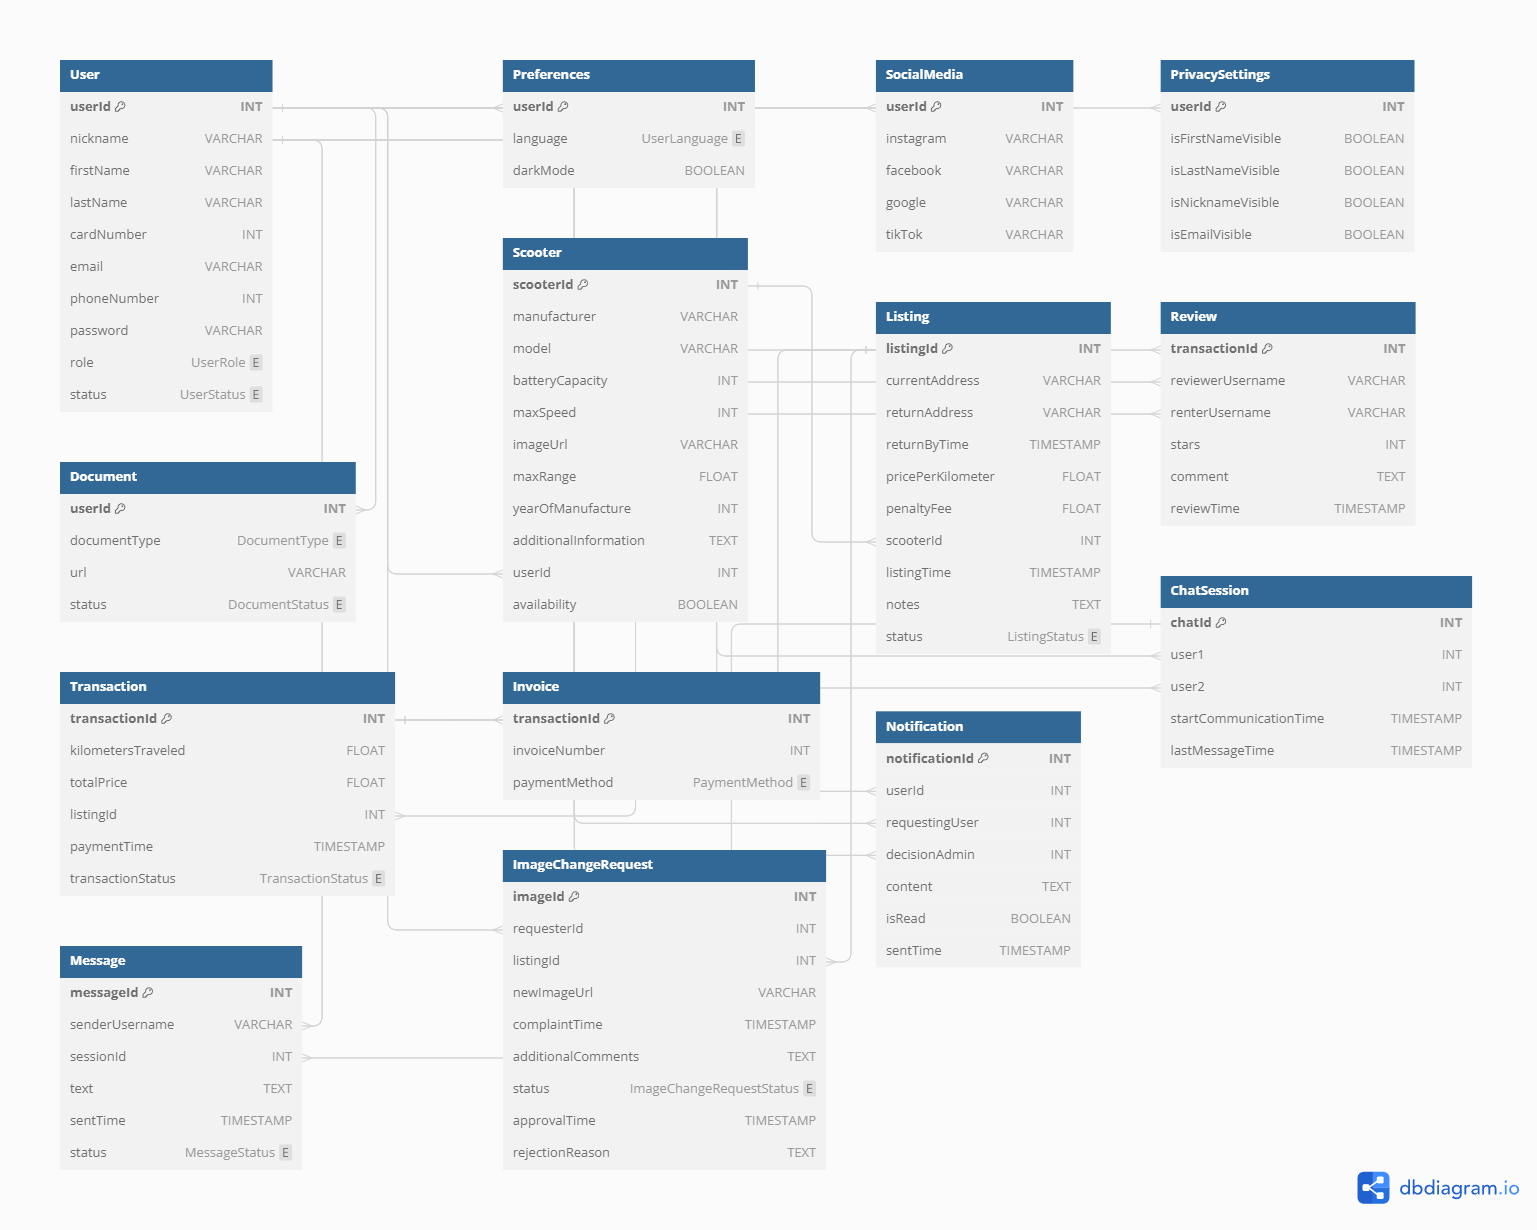
\includegraphics[width=0.5\linewidth]{bazapodataka.png}
	\caption{Slika dijagrama baze podataka}
	\label{fig:enter-label}
\end{figure}
